% ---------------------------------------------------------------------------
% Comparación de topologías: bus RS485 multipunto compartido frente a enlace
% RS422 punto a punto full-duplex.
%
% Compilar:  pdflatex diagrama_topologia_rs.tex
% ---------------------------------------------------------------------------
\documentclass[border=8pt]{standalone}
\usepackage[utf8]{inputenc}
\usepackage[T1]{fontenc}
\usepackage{lmodern}
\usepackage{tikz}
\usetikzlibrary{arrows.meta, calc}

\definecolor{cPropio}{HTML}{2A78D6}   % azul: lógica de diseño propio
\definecolor{cIP}{HTML}{EDA100}       % ámbar: IP de terceros
\definecolor{cExt}{HTML}{1BAF7A}      % aguamarina: software y hardware externo
\definecolor{cRef}{HTML}{8A8A85}      % gris: líneas, bandas y contornos

\begin{document}
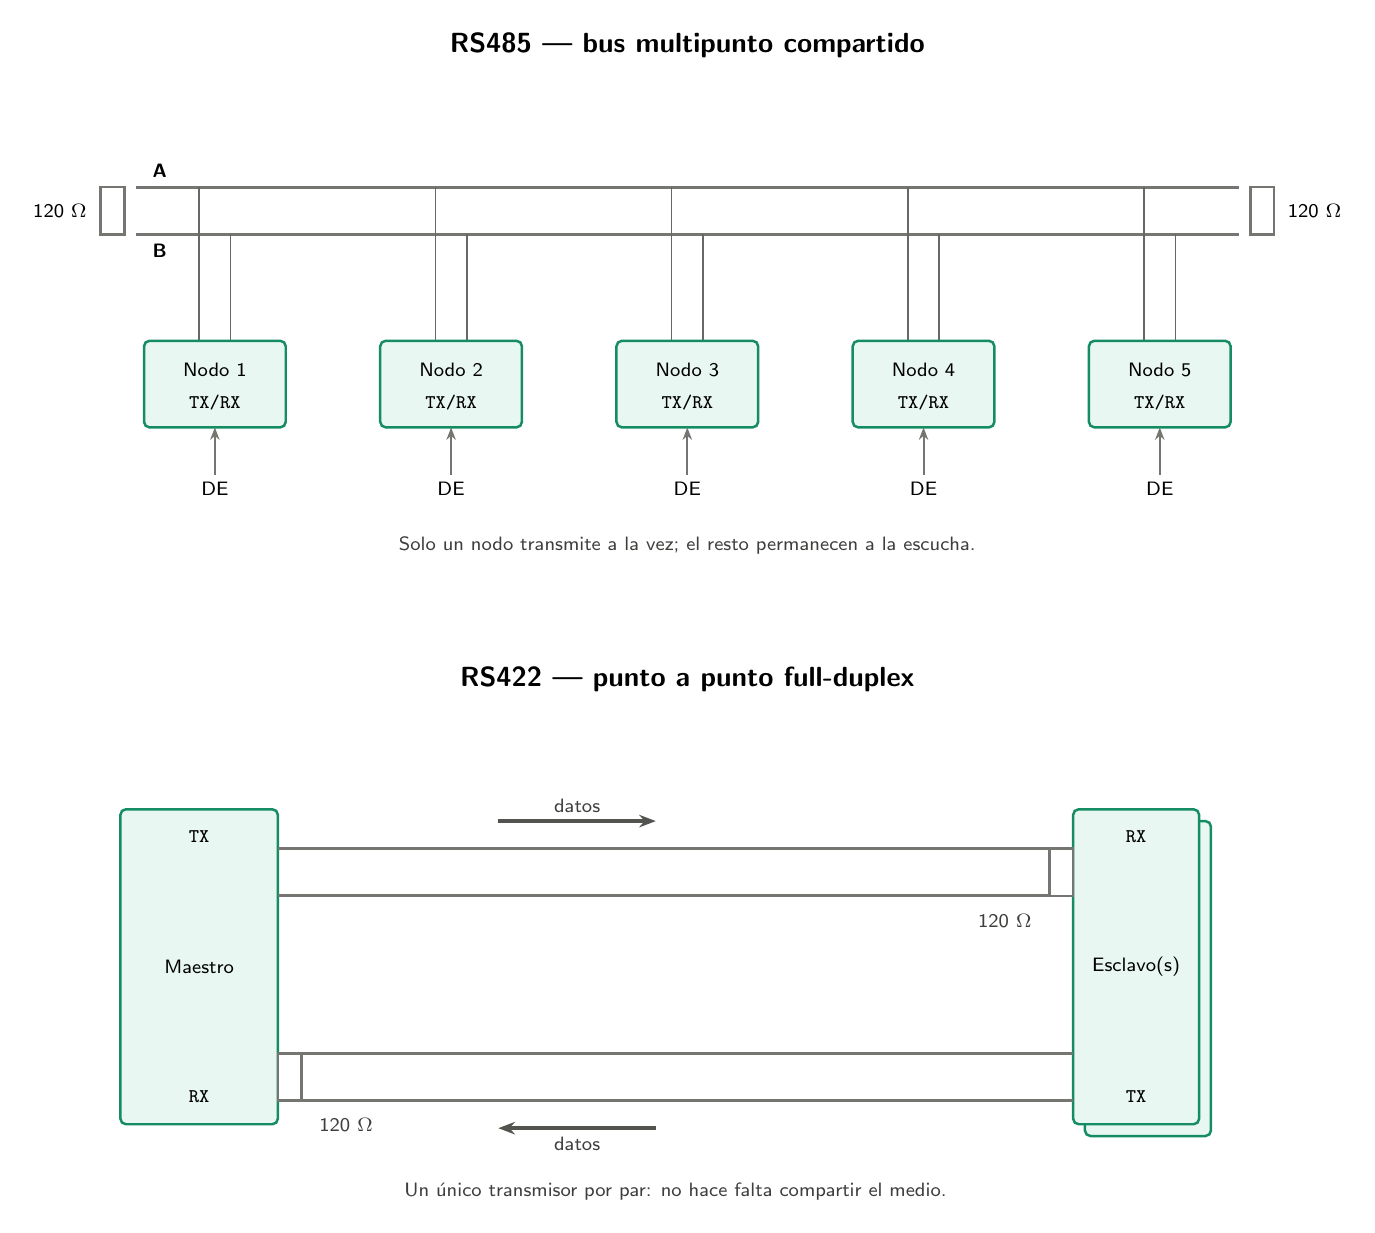
\begin{tikzpicture}[
    x=1cm, y=1cm, font=\sffamily\small,
    blk/.style={draw=cPropio, line width=0.9pt, rounded corners=2pt,
                fill=cPropio!7},
    ip/.style={draw=cIP!85!black, line width=0.9pt, rounded corners=2pt,
               fill=cIP!12},
    ext/.style={draw=cExt!80!black, line width=0.9pt, rounded corners=2pt,
                fill=cExt!10},
    band/.style={draw=cRef!45, dashed, line width=0.7pt, rounded corners=4pt},
    sig/.style={-{Stealth[length=4.5pt]}, line width=0.7pt, cRef!85!black},
    stream/.style={-{Stealth[length=6pt]}, line width=1.5pt, cRef!60!black},
    lbl/.style={font=\sffamily\scriptsize, inner sep=2pt},
    tlbl/.style={font=\ttfamily\scriptsize, inner sep=2pt},
    name/.style={font=\ttfamily\scriptsize, align=center},
    res/.style={draw=cRef!85!black, line width=0.9pt, fill=white},
]

% ===========================================================================
% (a) RS485 -- bus multipunto compartido
% ===========================================================================
\node[lbl, font=\sffamily\bfseries\normalsize] at (8.0,15.4)
      {RS485 --- bus multipunto compartido};

% ----- Líneas del bus -----
\draw[cRef!85!black, line width=1.1pt] (1.0,13.6) -- (15.0,13.6);
\draw[cRef!85!black, line width=1.1pt] (1.0,13.0) -- (15.0,13.0);
\node[lbl, anchor=south] at (1.3,13.65) {\textbf{A}};
\node[lbl, anchor=north] at (1.3,12.95) {\textbf{B}};

% ----- Terminaciones 120 ohm en los dos extremos -----
\draw[res] (0.55,13.0) rectangle (0.85,13.6);
\node[lbl, anchor=east] at (0.45,13.3) {120~$\Omega$};

\draw[res] (15.15,13.0) rectangle (15.45,13.6);
\node[lbl, anchor=west] at (15.55,13.3) {120~$\Omega$};

% ----- Nodos colgados del bus -----
\foreach \x/\n in {2/1, 5/2, 8/3, 11/4, 14/5} {
    % acometida diferencial: dos hilos, uno por cada línea del par
    \draw[cRef!75!black, line width=0.6pt] (\x-0.2,13.6) -- (\x-0.2,11.65);
    \draw[cRef!75!black, line width=0.6pt] (\x+0.2,13.0) -- (\x+0.2,11.65);
    % transceptor: mismo par para transmisión y recepción (half-duplex)
    \draw[ext] (\x-0.9,10.55) rectangle (\x+0.9,11.65);
    \node[lbl] at (\x,11.28) {Nodo \n};
    \node[tlbl] at (\x,10.86) {TX/RX};
    % habilitación de transmisión
    \draw[sig] (\x,9.95) -- (\x,10.55);
    \node[lbl, anchor=north] at (\x,9.93) {DE};
}

\node[lbl, text=cRef!45!black, align=center] at (8.0,9.05)
      {Solo un nodo transmite a la vez; el resto permanecen a la escucha.};

% ===========================================================================
% (b) RS422 -- punto a punto full-duplex
% ===========================================================================
\node[lbl, font=\sffamily\bfseries\normalsize] at (8.0,7.35)
      {RS422 --- punto a punto full-duplex};

% ----- Maestro -----
\draw[ext] (0.8,1.7) rectangle (2.8,5.7);
\node[lbl] at (1.8,3.7) {Maestro};
\node[tlbl] at (1.8,5.35) {TX};
\node[tlbl] at (1.8,2.05) {RX};

% ----- Esclavo(s): se dibuja más de un receptor posible -----
\draw[ext] (13.05,1.55) rectangle (14.65,5.55);
\draw[ext, fill=cExt!10] (12.9,1.7) rectangle (14.5,5.7);
\node[lbl] at (13.7,3.7) {Esclavo(s)};
\node[tlbl] at (13.7,5.35) {RX};
\node[tlbl] at (13.7,2.05) {TX};

% ----- Par de ida: TX del maestro -> RX del/de los esclavo(s) -----
\draw[cRef!85!black, line width=1.1pt] (2.8,5.2) -- (12.9,5.2);
\draw[cRef!85!black, line width=1.1pt] (2.8,4.6) -- (12.9,4.6);
\draw[stream] (5.6,5.55) -- (7.6,5.55);
\node[lbl, anchor=south, text=cRef!45!black] at (6.6,5.58) {datos};

% terminación en el extremo receptor (esclavo)
\draw[res] (12.6,4.6) rectangle (12.9,5.2);
\node[lbl, anchor=north east, text=cRef!45!black] at (12.45,4.45) {120~$\Omega$};

% ----- Par de vuelta: TX del/de los esclavo(s) -> RX del maestro -----
\draw[cRef!85!black, line width=1.1pt] (2.8,2.6) -- (12.9,2.6);
\draw[cRef!85!black, line width=1.1pt] (2.8,2.0) -- (12.9,2.0);
\draw[stream] (7.6,1.65) -- (5.6,1.65);
\node[lbl, anchor=north, text=cRef!45!black] at (6.6,1.62) {datos};

% terminación en el extremo receptor (maestro)
\draw[res] (2.8,2.0) rectangle (3.1,2.6);
\node[lbl, anchor=north west, text=cRef!45!black] at (3.25,1.85) {120~$\Omega$};

\node[lbl, text=cRef!45!black, align=center] at (7.85,0.85)
      {Un único transmisor por par: no hace falta compartir el medio.};

\end{tikzpicture}
\end{document}
